
%================================
\subsection{Resultados algoritmo concurrente por procesos}
\label{sec:Resultados algoritmo concurrente por procesos}

En esta sección se presentan los resultados obtenidos al ejecutar el algoritmo concurrente por procesos. Se realizaron pruebas utilizando diferentes tamaños de matrices y se midió el tiempo de ejecución para cada caso. Para este caso se aplicó la optimización por compilador usada tambien en el algoritmo secuencial, y se compararon los resultados con la versión sin optimización. A continuación, se muestran las tablas con los tiempos de ejecución y las gráficas correspondientes para analizar el rendimiento del algoritmo concurrente por procesos.

\begin{figure}[H]
      \centering
      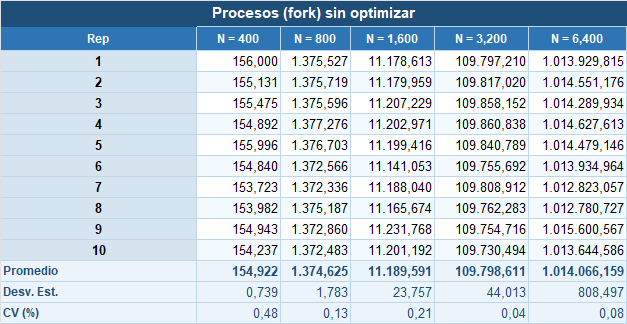
\includegraphics[width=0.8\textwidth]{images/tables/fork_noopt.png}
      \caption{Tiempos de ejecución del algoritmo concurrente por procesos para diferentes tamaños de matrices.}
      \label{fig:tiempos_procesos}
\end{figure}

\begin{figure}[H]
   \centering
   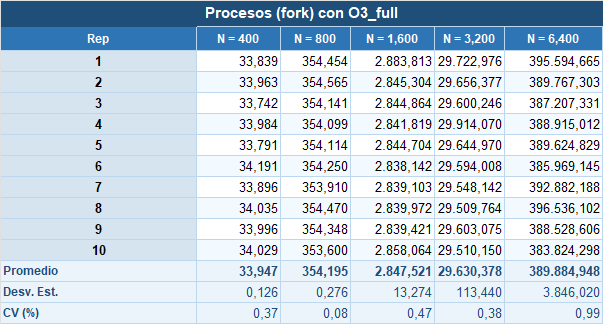
\includegraphics[width=1\textwidth]{images/tables/fork_opt.png}
   \caption{Tiempos de ejecución del algoritmo concurrente por procesos con optimizaciones.}
   \label{fig:tiempos_procesos_opt}
\end{figure}

\begin{figure}[H]
   \centering
   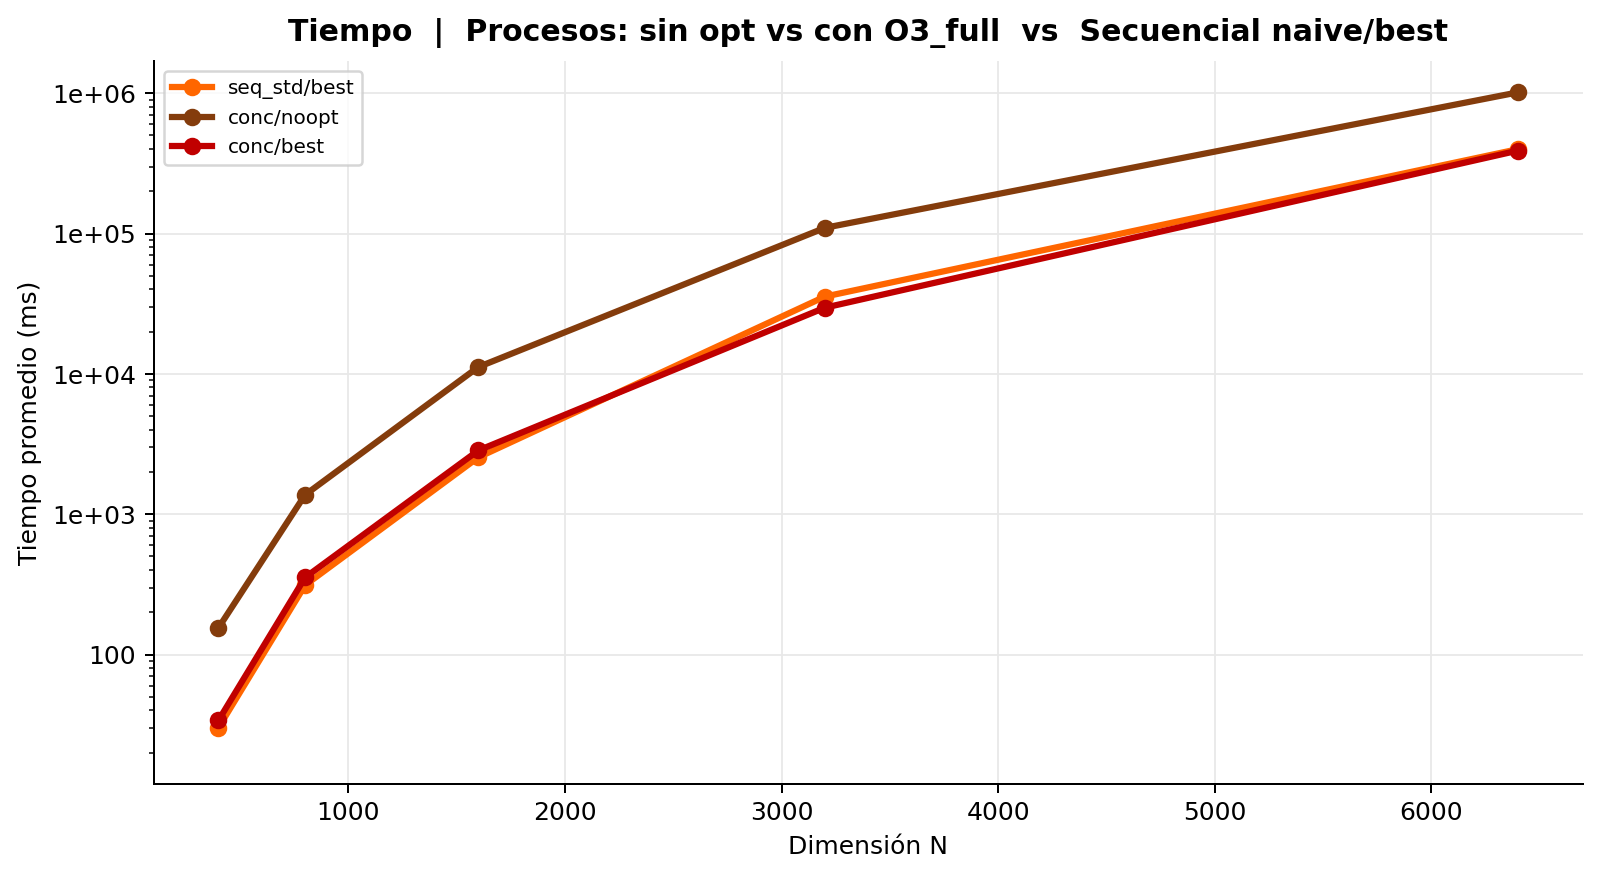
\includegraphics[width=1\textwidth]{images/charts/time_fork_noopt.png}
   \caption{Gráfica de tiempos de ejecución del algoritmo concurrente por procesos.}
   \label{fig:grafica_procesos}
\end{figure}

\begin{figure}[H]
   \centering
   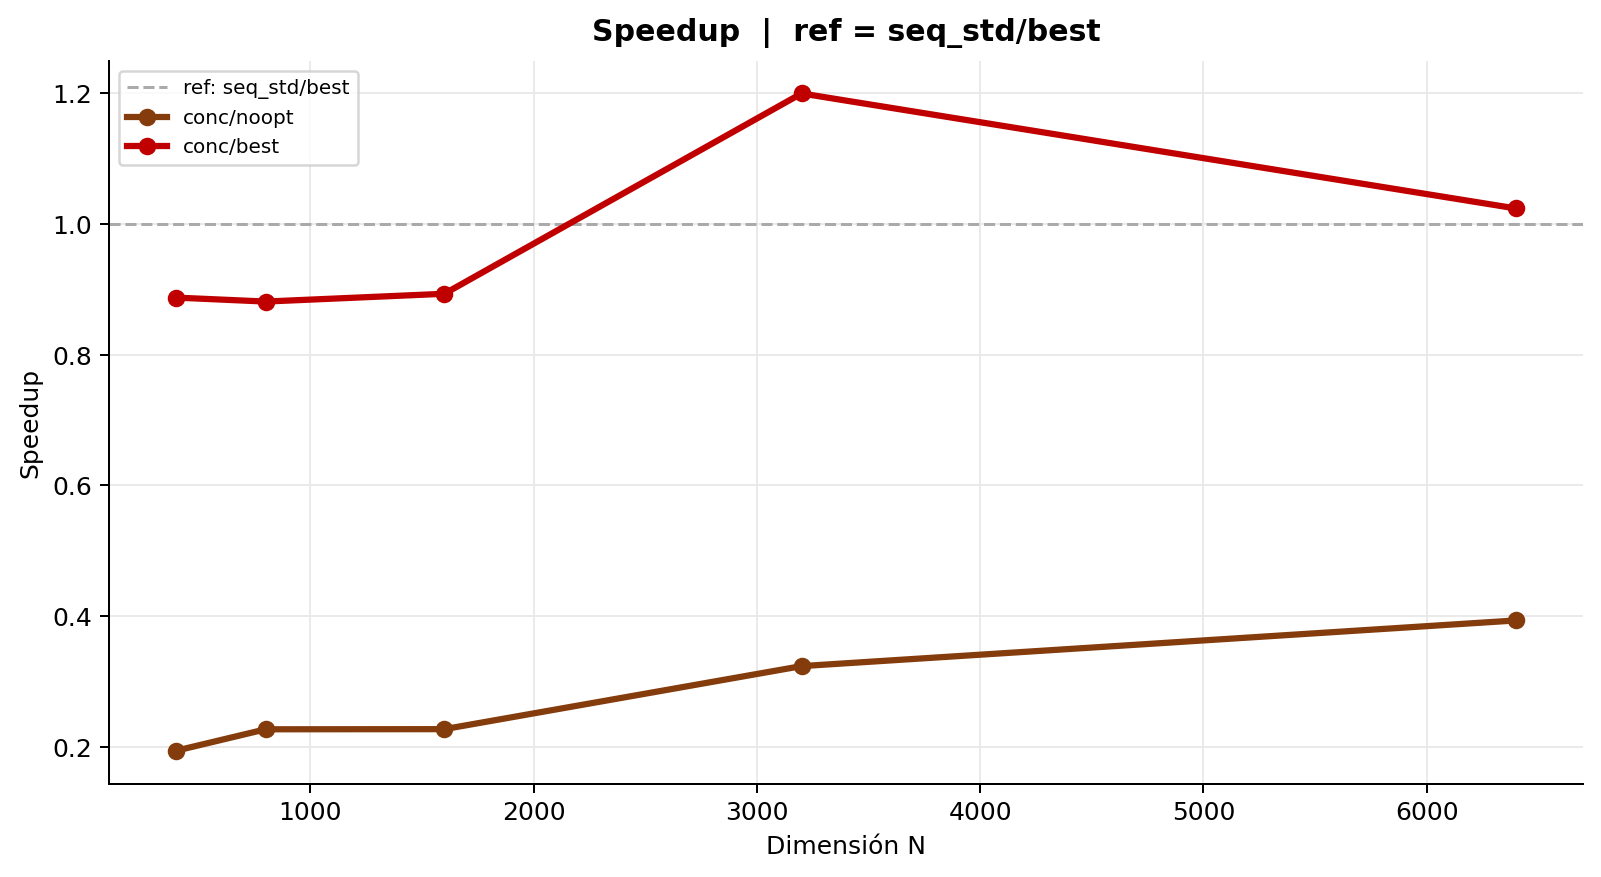
\includegraphics[width=1\textwidth]{images/charts/speedup_fork_noopt.png}
   \caption{Gráfica de Speedup del algoritmo concurrente por procesos.}
   \label{fig:speedup_procesos}  
\end{figure}

\begin{figure}[H]
   \centering
   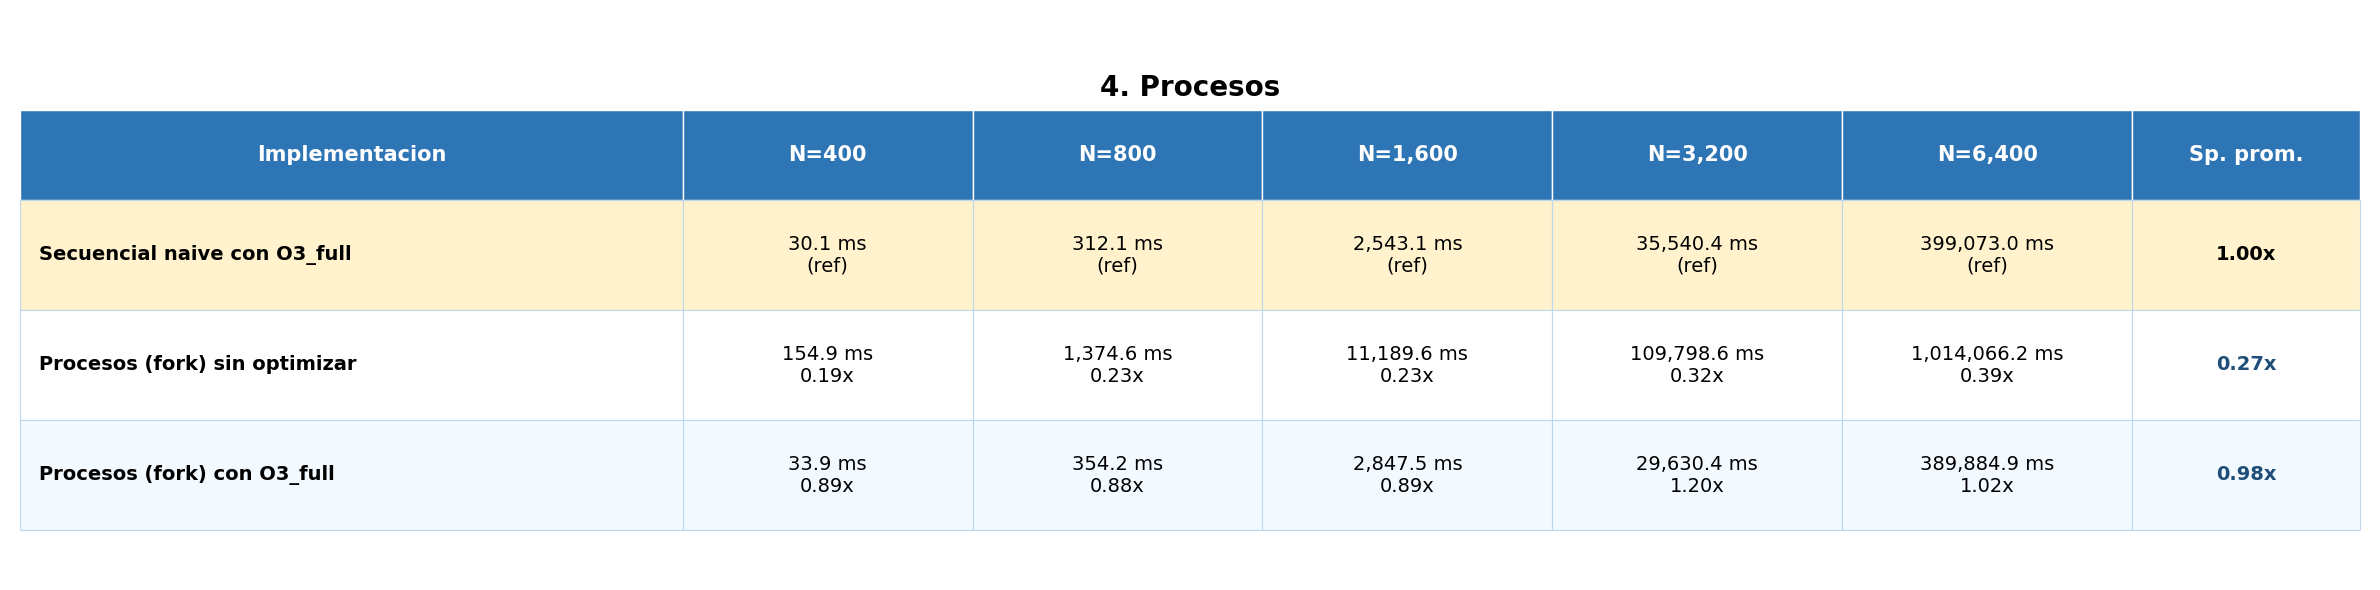
\includegraphics[width=1\textwidth]{images/tables/speedup_fork.png}
   \caption{Tabla de Speedup del algoritmo concurrente por procesos.}
   \label{fig:speedup_procesos}  
\end{figure}

En este caso se puede observar que el algoritmo concurrente por procesos no muestra una mejora significativa en el tiempo de ejecución en comparación con el algoritmo secuencial, especialmente para tamaños de matrices pequeñas. Aún si observamos la el speedup del algoritmo concurrente por procesos, no se aprecia una mejora en el rendimiento, lo que sugiere que la sobrecarga de crear y gestionar procesos puede estar afectando negativamente el rendimiento del algoritmo. Sin embargo, es importante destacar que para tamaños de matrices más grandes, el algoritmo concurrente por procesos podría mostrar una mejora en el rendimiento, aunque esto no se refleja claramente en los resultados obtenidos en este caso.